\documentclass[11pt,compress,t,notes=noshow, xcolor=table]{beamer}
\usepackage[]{graphicx}\usepackage[]{color}
% maxwidth is the original width if it is less than linewidth
% otherwise use linewidth (to make sure the graphics do not exceed the margin)
\makeatletter
\def\maxwidth{ %
  \ifdim\Gin@nat@width>\linewidth
    \linewidth
  \else
    \Gin@nat@width
  \fi
}
\makeatother

\newcommand{\citebutton}[2]{%
\beamergotobutton{\href{#2}{#1}}%
}

\newcommand{\blu}[1]{\textcolor{blue}{#1}}
\newcommand{\org}[1]{\textcolor{orange}{#1}}
\newcommand{\ques}{\textbf{\textcolor{red}{Question:  }}}
\newcommand{\questionssofar}{\begin{frame}\frametitle{Any questions?}\end{frame}}

\newcommand\warning{%
 \makebox[1.4em][c]{%
 \makebox[0pt][c]{\raisebox{.1em}{\scriptsize!}}%
 \makebox[0pt][c]{\color{red}\normalsize$\bigtriangleup$}}}%

\definecolor{fgcolor}{rgb}{0.345, 0.345, 0.345}
\newcommand{\hlnum}[1]{\textcolor[rgb]{0.686,0.059,0.569}{#1}}%
\newcommand{\hlstr}[1]{\textcolor[rgb]{0.192,0.494,0.8}{#1}}%
\newcommand{\hlcom}[1]{\textcolor[rgb]{0.678,0.584,0.686}{\textit{#1}}}%
\newcommand{\hlopt}[1]{\textcolor[rgb]{0,0,0}{#1}}%
\newcommand{\hlstd}[1]{\textcolor[rgb]{0.345,0.345,0.345}{#1}}%
\newcommand{\hlkwa}[1]{\textcolor[rgb]{0.161,0.373,0.58}{\textbf{#1}}}%
\newcommand{\hlkwb}[1]{\textcolor[rgb]{0.69,0.353,0.396}{#1}}%
\newcommand{\hlkwc}[1]{\textcolor[rgb]{0.333,0.667,0.333}{#1}}%
\newcommand{\hlkwd}[1]{\textcolor[rgb]{0.737,0.353,0.396}{\textbf{#1}}}%
\let\hlipl\hlkwb

\usepackage{framed}
\makeatletter
\newenvironment{kframe}{%
 \def\at@end@of@kframe{}%
 \ifinner\ifhmode%
  \def\at@end@of@kframe{\end{minipage}}%
  \begin{minipage}{\columnwidth}%
 \fi\fi%
 \def\FrameCommand##1{\hskip\@totalleftmargin \hskip-\fboxsep
 \colorbox{shadecolor}{##1}\hskip-\fboxsep
     % There is no \\@totalrightmargin, so:
     \hskip-\linewidth \hskip-\@totalleftmargin \hskip\columnwidth}%
 \MakeFramed {\advance\hsize-\width
   \@totalleftmargin\z@ \linewidth\hsize
   \@setminipage}}%
 {\par\unskip\endMakeFramed%
 \at@end@of@kframe}
\makeatother

\definecolor{shadecolor}{rgb}{.97, .97, .97}
\definecolor{messagecolor}{rgb}{0, 0, 0}
\definecolor{warningcolor}{rgb}{1, 0, 1}
\definecolor{errorcolor}{rgb}{1, 0, 0}
\newenvironment{knitrout}{}{} % an empty environment to be redefined in TeX

\usepackage{alltt}
\newcommand{\SweaveOpts}[1]{}  % do not interfere with LaTeX
\newcommand{\SweaveInput}[1]{} % because they are not real TeX commands
\newcommand{\Sexpr}[1]{}       % will only be parsed by R
\newcommand{\xmark}{\ding{55}}%


\usepackage[english]{babel}
\usepackage[utf8]{inputenc}

\usepackage{dsfont}
\usepackage{verbatim}
\usepackage{amsmath}
\usepackage{amsfonts}
\usepackage{amssymb}
\usepackage{bm}
\usepackage{csquotes}
\usepackage{multirow}
\usepackage{longtable}
\usepackage{booktabs}
\usepackage{enumerate}
\usepackage[absolute,overlay]{textpos}
\usepackage{psfrag}
\usepackage{algorithm}
\usepackage{algpseudocode}
\usepackage{eqnarray}
\usepackage{arydshln}
\usepackage{tabularx}
\usepackage{placeins}
\usepackage{tikz}
\usepackage{setspace}
\usepackage{colortbl}
\usepackage{mathtools}
\usepackage{wrapfig}
\usepackage{bm}
\usepackage{amsmath}
\usepackage{pifont}

\usetikzlibrary{shapes.multipart,shapes,arrows,automata,positioning,calc,chains,trees, shadows}
\tikzset{
  %Define standard arrow tip
  >=stealth',
  %Define style for boxes
  punkt/.style={
    rectangle,
    rounded corners,
    draw=black, very thick,
    text width=6.5em,
    minimum height=2em,
    text centered},
  % Define arrow style
  pil/.style={
    ->,
    thick,
    shorten <=2pt,
    shorten >=2pt,}
}

\tikzstyle{vec}=[draw, rectangle, fill = white, minimum width=5mm, minimum height=1cm, inner sep = 2pt]

\usepackage{subfig}

% Defines macros and environments
\usepackage{../../style/lmu-lecture}


\let\code=\texttt
\let\proglang=\textsf

\setkeys{Gin}{width=0.9\textwidth}

\setbeamertemplate{frametitle}{\expandafter\uppercase\expandafter\insertframetitle}

\usepackage{bbm}
% basic latex stuff
\newcommand{\pkg}[1]{{\fontseries{b}\selectfont #1}} %fontstyle for R packages
\newcommand{\lz}{\vspace{0.5cm}} %vertical space
\newcommand{\dlz}{\vspace{1cm}} %double vertical space
\newcommand{\oneliner}[1] % Oneliner for important statements
{\begin{block}{}\begin{center}\begin{Large}#1\end{Large}\end{center}\end{block}}


%new environments
\newenvironment{vbframe}  %frame with breaks and verbatim
{
 \begin{frame}[containsverbatim,allowframebreaks]
}
{
\end{frame}
}

\newenvironment{vframe}  %frame with verbatim without breaks (to avoid numbering one slided frames)
{
 \begin{frame}[containsverbatim]
}
{
\end{frame}
}

\newenvironment{blocki}[1]   % itemize block
{
 \begin{block}{#1}\begin{itemize}
}
{
\end{itemize}\end{block}
}

\newenvironment{fragileframe}[2]{  %fragile frame with framebreaks
\begin{frame}[allowframebreaks, fragile, environment = fragileframe]
\frametitle{#1}
#2}
{\end{frame}}


\newcommand{\myframe}[2]{  %short for frame with framebreaks
\begin{frame}[allowframebreaks]
\frametitle{#1}
#2
\end{frame}}

\newcommand{\remark}[1]{
  \textbf{Remark:} #1
}


\newenvironment{deleteframe}
{
\begingroup
\usebackgroundtemplate{
\includegraphics[width=\paperwidth,height=\paperheight]{../style/color/red.png}}
 \begin{frame}
}
{
\end{frame}
\endgroup
}
\newenvironment{simplifyframe}
{
\begingroup
\usebackgroundtemplate{
\includegraphics[width=\paperwidth,height=\paperheight]{../style/color/yellow.png}}
 \begin{frame}
}
{
\end{frame}
\endgroup
}\newenvironment{draftframe}
{
\begingroup
\usebackgroundtemplate{
\includegraphics[width=\paperwidth,height=\paperheight]{../style/color/green.jpg}}
 \begin{frame}
}
{
\end{frame}
\endgroup
}
% https://tex.stackexchange.com/a/261480: textcolor that works in mathmode
\makeatletter
\renewcommand*{\@textcolor}[3]{%
  \protect\leavevmode
  \begingroup
    \color#1{#2}#3%
  \endgroup
}
\makeatother





\input{../../latex-math/basic-math.tex}
\input{../../latex-math/basic-ml.tex}

%\newcommand{\titlefigure}{figure/gpt_sq.png}
\newcommand{\learninggoals}{
\item Understand the concept of regularization
\item Understand L2 regularization in more detail}

\title{Deep Learning basics}
% \author{}
\institute{\href{https://slds-lmu.github.io/lecture_dl4nlp/}{slds-lmu.github.io/lecture\_dl4nlp}}
\date{}

\begin{document}
\lecturechapter{Backpropagation}
\lecture{Deep Learning for NLP}

% ------------------------------------------------------------------------------

\begin{vbframe}{}

\vfill

\begin{itemize}
\item Forward propagation: Input information $\vec x$ propagates through network to produce output $\hat y$ (and cost $J(\vec\theta)$ in training)
\item Back-propagation: 
\begin{itemize}
 \item compute gradient w.r.t. model parameters
 \item Cost gradient propagates backwards through the network
\end{itemize}
\item Back-propagation is part of learning procedure (e.g. stochastic gradient descent), not learning procedure in itself.

\end{itemize}
\begin{center}
%\includegraphics[width = 0.5\textwidth]{./}
\end{center}

\vfill

\end{vbframe}


% ------------------------------------------------------------------------------

\begin{vbframe}{Chain Rule of Calculus: Real Functions}

\vfill

\begin{itemize}
\item Let
$$x, y, z \in \mathbb{R}$$
$$f, g : \mathbb{R} \rightarrow \mathbb{R}$$
$$y = g(x)$$
$$z = f(g(x)) = f(y)$$
\item Then
$$\frac{dz}{dx} = \frac{dz}{dy} \frac{dy}{dx}$$
\end{itemize}
\begin{center}
%\includegraphics[width = 0.5\textwidth]{./}
\end{center}

\vfill

\end{vbframe}


% ------------------------------------------------------------------------------

\begin{vbframe}{Chain Rule of Calculus: Multivariate Functions}

\vfill

\begin{itemize}
\item Let
$$\vec x \in \mathbb{R}^m, \vec y \in \mathbb{R}^n, z \in \mathbb{R}$$
$$f : \mathbb{R}^n \rightarrow \mathbb{R}$$
$$g : \mathbb{R}^m \rightarrow \mathbb{R}^n$$
$$\vec y = g(\vec x)$$
$$z = f(g(\vec x)) = f(\vec y)$$
\item Then
$$\frac{\partial z}{\partial x_i} = 
		\frac{\partial z}{\partial y_1} \frac{\partial y_1}{\partial x_i} +
		\frac{\partial z}{\partial y_2} \frac{\partial y_2}{\partial x_i} + \ldots +
		\frac{\partial z}{\partial y_n} \frac{\partial y_n}{\partial x_i} =
\sum_{j=1}^n \frac{\partial z}{\partial y_j} \frac{\partial y_j}{\partial x_i}$$
\item In order to write this in vector notation, we need to define the Jacobian matrix.
\end{itemize}
\begin{center}
%\includegraphics[width = 0.5\textwidth]{./}
\end{center}


\vfill

\end{vbframe}


% ------------------------------------------------------------------------------

\begin{vbframe}{Jacobian}

\vfill

\begin{itemize}
\item The Jacobian matrix is the matrix of all first-order partial derivatives of a vector-valued function. 
\[\vec J = \frac{\partial \vec g(\vec x)}{\partial \vec x} =
\begin{bmatrix}
    \frac{\partial g(\vec x)_1}{\partial x_1} & \cdots & \frac{\partial g(\vec x)_1}{\partial x_m} \\
    & & \\
    \frac{\partial g(\vec x)_2}{\partial x_1} & & \frac{\partial g(\vec x)_2}{\partial x_m}\\
    \vdots & \ddots & \vdots \\
    & &  \\
    \frac{\partial g(\vec x)_n}{\partial x_1}& \cdots &  \frac{\partial g(\vec x)_n}{\partial x_m} \\
\end{bmatrix} 
\]
\item How to write in terms of gradients?

\item We can write the chain rule as:\\
\vspace{.2cm}
%$\displaystyle{\nabla_{\vec x} z = }$ \pause $\displaystyle{\left(\nabla_{\vec y} z\right)^T \frac{\partial \vec y}{\partial \vec x}}$
$\displaystyle{\nabla_{\vec x} z = }$ \pause $\displaystyle{\left(\frac{\partial \vec y}{\partial \vec x}\right)^T \nabla_{\vec y} z}$

\end{itemize}
\begin{center}
%\includegraphics[width = 0.5\textwidth]{./}
\end{center}

\vfill

\end{vbframe}


% ------------------------------------------------------------------------------

\begin{vbframe}{Viewing the Network as a Graph}

\vfill

\begin{itemize}
\item Nodes are function outputs (can be scalar or vector valued)
\item Arrows are inputs
\item Example: Scalar multiplication $z = x y$.
\end{itemize}
\begin{center}
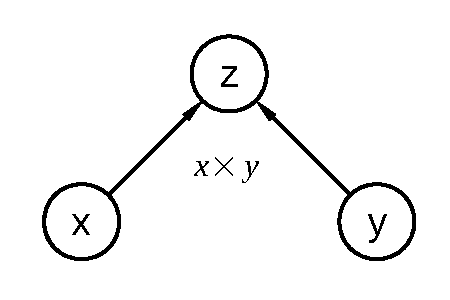
\includegraphics[width = 0.3\textwidth]{./figure/simple_mult_graph}
\end{center}

\vfill

\end{vbframe}


% ------------------------------------------------------------------------------

\begin{vbframe}{Which Function?}

\vfill

\begin{center}
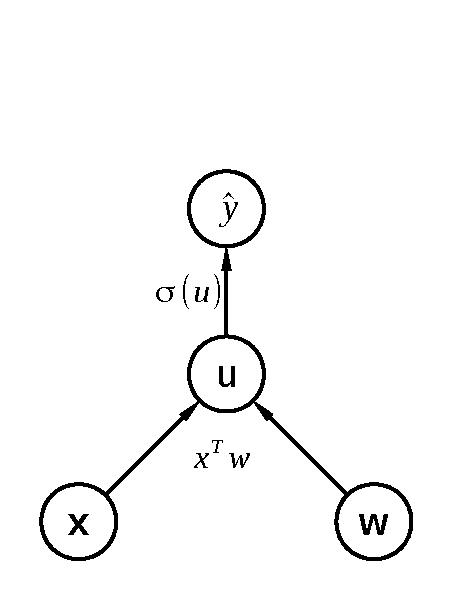
\includegraphics[width = 0.4\textwidth]{./figure/sigmoid_graph}
\end{center}

\vfill

\end{vbframe}


% ------------------------------------------------------------------------------

\begin{vbframe}{Graph with Cost}

\vfill

\begin{center}
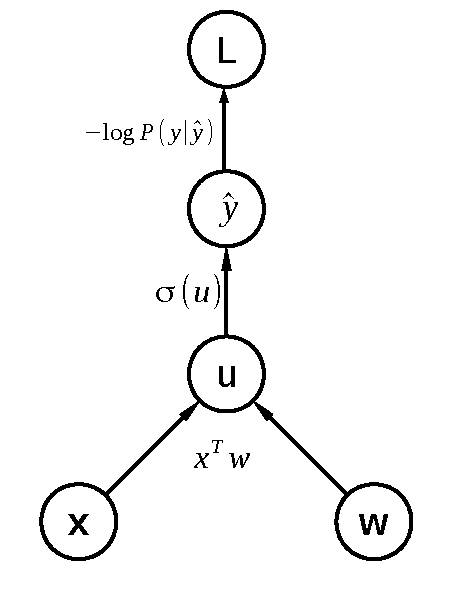
\includegraphics[width = 0.4\textwidth]{./figure/sigmoid_graph_with_loss}
\end{center}

\vfill

\end{vbframe}


% ------------------------------------------------------------------------------

\begin{vbframe}{Which Function?}

\vfill

\begin{itemize}
\item Parameter vectors can be converted to matrix as needed.
\end{itemize}
\begin{center}
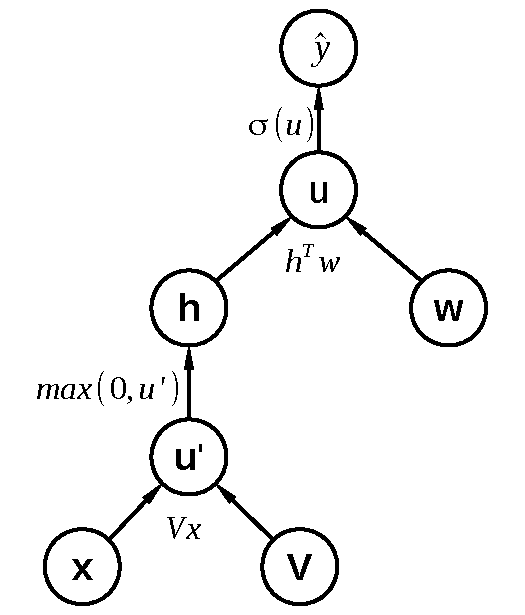
\includegraphics[width = 0.4\textwidth]{./figure/relu_sigmoid_graph}
\end{center}

\vfill

\end{vbframe}


% ------------------------------------------------------------------------------

\begin{vbframe}{Forward Pass}

\vfill

\begin{itemize}
\item Green: known or computed.
\end{itemize}
\begin{center}
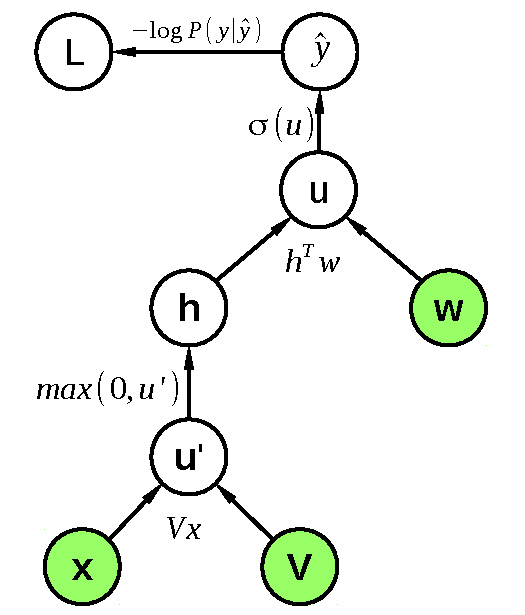
\includegraphics[width = 0.4\textwidth]{./figure/relu_sigmoid_graph_with_loss1}
\end{center}

\vfill

\end{vbframe}


% ------------------------------------------------------------------------------

\begin{vbframe}{Forward Pass}

\vfill

\begin{itemize}
\item Green: known or computed.
\end{itemize}
\begin{center}
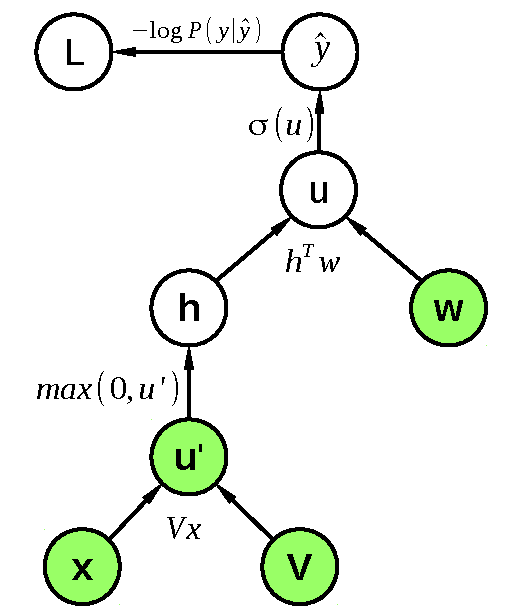
\includegraphics[width = 0.4\textwidth]{./figure/relu_sigmoid_graph_with_loss2}
\end{center}

\vfill

\end{vbframe}


% ------------------------------------------------------------------------------

\begin{vbframe}{Forward Pass}

\vfill

\begin{itemize}
\item Green: known or computed.
\end{itemize}
\begin{center}
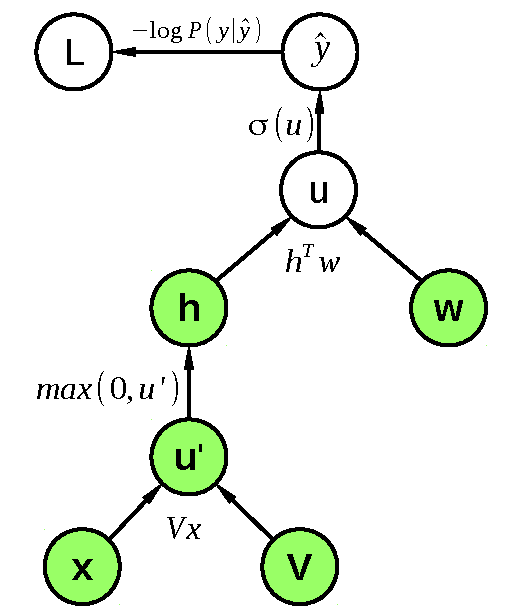
\includegraphics[width = 0.4\textwidth]{./figure/relu_sigmoid_graph_with_loss3}
\end{center}

\vfill

\end{vbframe}


% ------------------------------------------------------------------------------

\begin{vbframe}{Forward Pass}

\vfill

\begin{itemize}
\item End of forward pass (some steps skipped).
\end{itemize}
\begin{center}
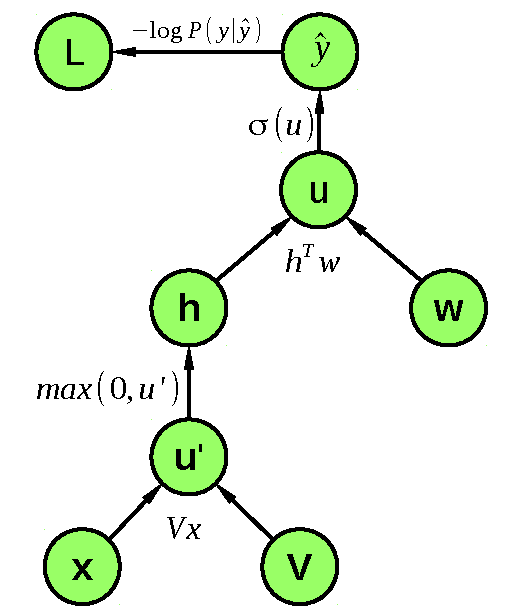
\includegraphics[width = 0.4\textwidth]{./figure/relu_sigmoid_graph_with_loss4}
\end{center}

\vfill

\end{vbframe}


% ------------------------------------------------------------------------------

\begin{vbframe}{Backward Pass}

\vfill

\begin{itemize}
\item Red: gradient of cost computed for node.
\end{itemize}
\begin{center}
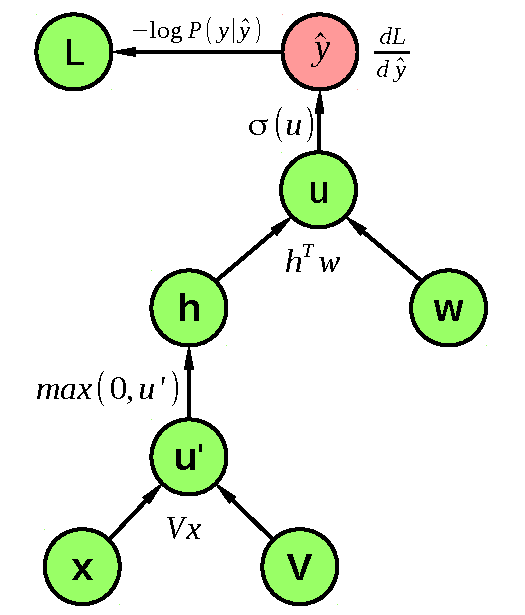
\includegraphics[width = 0.4\textwidth]{./figure/relu_sigmoid_graph_with_loss_backward}
\end{center}

\vfill

\end{vbframe}


% ------------------------------------------------------------------------------

\begin{vbframe}{Backward Pass}

\vfill

\begin{itemize}
\item Red: gradient of cost computed for node.
\end{itemize}
\begin{center}
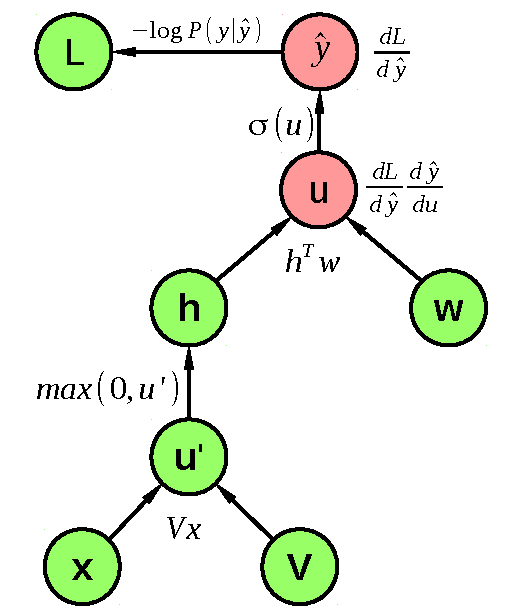
\includegraphics[width = 0.4\textwidth]{./figure/relu_sigmoid_graph_with_loss_backward2}
\end{center}

\vfill

\end{vbframe}


% ------------------------------------------------------------------------------

\begin{vbframe}{Backward Pass}

\vfill

\begin{itemize}
\item Red: gradient of cost computed for node.
\end{itemize}
\begin{center}
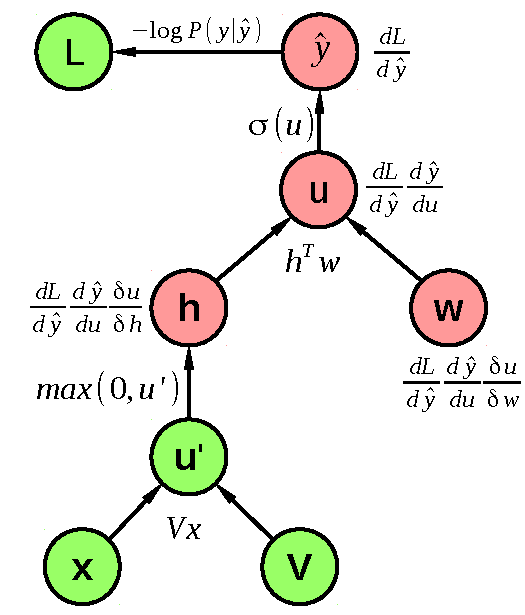
\includegraphics[width = 0.4\textwidth]{./figure/relu_sigmoid_graph_with_loss_backward3}
\end{center}

\vfill

\end{vbframe}


% ------------------------------------------------------------------------------

\begin{vbframe}{Backward Pass}

\vfill

\begin{itemize}
\item We have the gradients for all parameters, let's use them for SGD.
\end{itemize}
\begin{center}
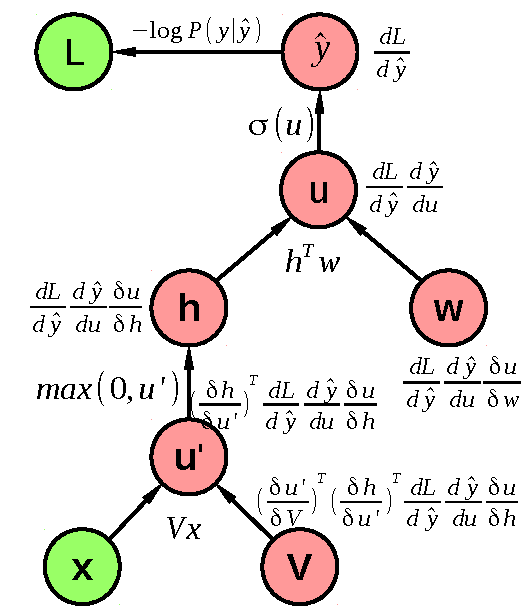
\includegraphics[width = 0.4\textwidth]{./figure/relu_sigmoid_graph_with_loss_backward4}
\end{center}

\vfill

\end{vbframe}


\endlecture
\end{document}
